\documentclass[conference,a4paper]{IEEEtran}
\usepackage[utf8]{inputenc}
\usepackage[T1]{fontenc}
\usepackage[spanish,es-noshorthands,es-tabla]{babel}
\usepackage{amsmath,amssymb}
\usepackage{graphicx}
\usepackage{booktabs}
\usepackage{siunitx}
\sisetup{output-decimal-marker={.}}
\usepackage{listings}
\usepackage{xcolor}
\usepackage[hidelinks]{hyperref}
\lstset{basicstyle=\ttfamily\scriptsize, breaklines=true, frame=single, columns=fullflexible,
        keywordstyle=\color{blue!60!black}, commentstyle=\color{green!40!black}, language=C++}
\graphicspath{{figuras/}}

\raggedbottom
\begin{document}

\title{Implementación de un Observador de Luenberger y un Filtro de Kalman Lineal para Estimar la Corriente y la Velocidad de un Motor DC}

\author{\IEEEauthorblockN{Andrés Ramírez\qquad Simón Patiño\qquad Jeronimo Valencia\\ Jorge Alejandro de Santiago}
\IEEEauthorblockA{Ingeniería Mecatrónica -- Control Digital\\
Universidad EIA, Envigado, Colombia}}

\maketitle

\begin{abstract}
Se diseñan e implementan dos observadores de estado discretos, un observador de Luenberger de orden completo tipo predictor y un filtro de Kalman lineal, para estimar la corriente de armadura y la velocidad de un motorreductor Pololu 37D \#4753 (50:1) midiendo únicamente la velocidad con un encoder incremental. El modelo paramétrico del laboratorio anterior se ajusta para que a \SI{12}{V} entregue \SI{0.2}{A} y la velocidad nominal, y se afina con escalones medidos en el codo de un robot SCARA. Ambos observadores se implementan en una Raspberry Pi Pico con un periodo de muestreo de \SI{10}{ms} y se evalúan ante escalones, cambios de referencia y perturbaciones de carga. Los dos estiman de forma coherente la corriente; el filtro de Kalman sigue la velocidad con un error de \SI{7.8}{rad/s} RMS bajo perturbaciones, frente a \SI{34.8}{rad/s} del observador de Luenberger.
\end{abstract}

\begin{IEEEkeywords}
Observador de Luenberger, filtro de Kalman, motor DC, espacio de estados, Raspberry Pi Pico.
\end{IEEEkeywords}

\section{Introducción}
En muchas aplicaciones no todas las variables de un sistema se pueden medir, ya sea porque no hay un sensor disponible o porque medirlas es costoso. En un motor DC la velocidad se obtiene fácilmente con un encoder, pero la corriente de armadura requiere un sensor adicional. Un observador de estados permite reconstruir los estados no medidos a partir del modelo del sistema, de la entrada y de las salidas medidas \cite{ogata}.

En este trabajo se implementan los dos observadores propuestos en la guía del laboratorio \cite{guia,guiaeia}: el observador de Luenberger, diseñado por asignación de polos con la fórmula de Ackermann, y el filtro de Kalman lineal, diseñado a partir de la incertidumbre del modelo y de la medición \cite{welch}. A diferencia de la guía, que usa una tarjeta myRIO y LabVIEW, la implementación se hace en una Raspberry Pi Pico sobre el motor del codo de un robot SCARA.

\section{Marco teórico}
\subsection{Modelo del motor DC}
Con los estados $x=[i_a\;\;\omega]^T$, la entrada $u=V_a$ y la salida medida $y=\omega$, las ecuaciones del motor son
\begin{align}
\dot{i}_a &= -\frac{R_a}{L_a} i_a - \frac{K_v}{L_a}\omega + \frac{1}{L_a}V_a,\\
\dot{\omega} &= \frac{K_v}{J} i_a - \frac{\beta}{J}\omega,
\end{align}
es decir, $\dot{x}=A_c x + B_c u$, $y = Cx$ con
\begin{equation}
A_c=\begin{bmatrix}-\frac{R_a}{L_a} & -\frac{K_v}{L_a}\\[2pt] \frac{K_v}{J} & -\frac{\beta}{J}\end{bmatrix},\quad
B_c=\begin{bmatrix}\frac{1}{L_a}\\[2pt] 0\end{bmatrix},\quad
C=\begin{bmatrix}0 & 1\end{bmatrix}.
\end{equation}

\subsection{Discretización}
Con un retenedor de orden cero y periodo $T_s$:
\begin{equation}
A = e^{A_c T_s},\qquad B=\int_0^{T_s} e^{A_c\tau}\,d\tau\, B_c,
\end{equation}
\begin{equation}
x_k = A x_{k-1} + B u_{k-1},\qquad y_k = C x_k .
\end{equation}

\subsection{Observador de Luenberger}
El observador de orden completo tipo predictor usa la entrada y la medición del instante anterior:
\begin{equation}
\hat{x}_k = (A-LC)\hat{x}_{k-1} + L\,y_{k-1} + B\,u_{k-1}.
\label{eq:luen}
\end{equation}
El error de estimación evoluciona como $e_k=(A-LC)e_{k-1}$, de modo que $L$ se elige para que los valores propios de $A-LC$ estén dentro del círculo unitario. Con la fórmula de Ackermann:
\begin{equation}
L = \Phi(A)\,\mathcal{O}^{-1}\begin{bmatrix}0\\1\end{bmatrix},\qquad \mathcal{O}=\begin{bmatrix}C\\CA\end{bmatrix},
\end{equation}
donde $\Phi(z)$ es el polinomio característico deseado.

\subsection{Filtro de Kalman lineal}
Partiendo de $\hat{x}_0$ y $P_0$, en cada muestra se hace una predicción y una corrección \cite{welch}:
\begin{align}
\hat{x}_k^- &= A\hat{x}_{k-1}^+ + B u_{k-1}, & P_k^- &= A P_{k-1}^+ A^T + Q,\\
K_k &= P_k^- C^T (C P_k^- C^T + R)^{-1}, & &\\
\hat{x}_k^+ &= \hat{x}_k^- + K_k(y_k - C\hat{x}_k^-), & P_k^+ &= (I-K_kC)P_k^- ,
\end{align}
donde $Q$ representa la incertidumbre del modelo y $R$ la varianza de la medición.

\section{Montaje experimental}
Se usa el motor del codo de un SCARA RRP: un motorreductor Pololu 37D \#4753 de \SI{12}{V} con caja 50:1 \cite{pololu} que mueve el antebrazo mediante una polea 3:1. El encoder Hall da 64 cuentas por vuelta del eje del motor; la velocidad se calcula como la diferencia de posición entre dos muestras dividida por $T_s$, por lo que su resolución es de $2\pi/(64\,T_s)\approx\SI{9.8}{rad/s}$. El motor se alimenta con un puente H BTS7960 controlado por PWM a \SI{20}{kHz} desde una Raspberry Pi Pico, que lee el encoder con una máquina de estados PIO.

El firmware ejecuta un lazo cada $T_s=\SI{10}{ms}$ en el que mide la velocidad, actualiza los dos observadores y aplica el voltaje del experimento; los datos se envían por USB y un script de Python los guarda y grafica. Como el codo tiene un recorrido limitado (unos \SI{3.7}{rad}), el firmware hace un \emph{home} contra el final de carrera, corta el voltaje antes de los extremos y detiene el motor si queda bloqueado. El hombro y el eje prismático se mantienen frenados.

\section{Modelo del motor}
\subsection{Modelo del Laboratorio 1}
La identificación paramétrica previa daba la matriz $A_c$ de la Tabla~\ref{tab:param} (columna Lab~1), con una resistencia de armadura de \SI{72.7}{\ohm}. Con ese modelo, a \SI{12}{V} el motor llega a \SI{0.084}{A} y \SI{558}{rad/s} (\SI{107}{rpm} a la salida), lejos de los \SI{0.2}{A} y \SI{200}{rpm} que especifica el fabricante. $K_v$ y $\beta$ eran coherentes con el datasheet, pero $R_a$ era unas 30 veces mayor que el valor que se deduce de la corriente de arranque (\SI{5.5}{A} a \SI{12}{V}).

\subsection{Ajuste del modelo}
Se fijó $R_a = 12/5.5 = \SI{2.18}{\ohm}$ y se impusieron las dos condiciones de la guía en estado estable, $i_a=\SI{0.2}{A}$ y $\omega=\omega_{nom}=\SI{1047}{rad/s}$ (\SI{10000}{rpm} en el eje del motor), de donde
\begin{equation}
K_v=\frac{12-R_a\,i_a}{\omega_{nom}},\qquad \beta = \frac{K_v\, i_a}{\omega_{nom}}.
\end{equation}
Luego se ajustaron $J$ y $L_a$ por mínimos cuadrados para reproducir tres escalones de 4, 6 y \SI{8}{V} medidos en el codo. El valor de $J$ resultante incluye la inercia del antebrazo reflejada al eje del motor. La Tabla~\ref{tab:param} resume los parámetros.

\begin{table}[!t]
\centering
\caption{Parámetros del motor}
\label{tab:param}
\begin{tabular}{lcc}
\toprule
Parámetro & Lab 1 & Ajustado \\
\midrule
$R_a$ (\si{\ohm}) & 72.7 & 2.18 \\
$L_a$ (\si{H}) & \num{6.62e-2} & \num{5.56e-4} \\
$K_v$ (\si{V.s/rad}) & \num{1.06e-2} & \num{1.104e-2} \\
$J$ (\si{kg.m^2}) & \num{8.55e-7} & \num{2.81e-6} \\
$\beta$ (\si{N.m.s}) & \num{1.59e-6} & \num{2.11e-6} \\
\midrule
$i_a$ a \SI{12}{V} (\si{A}) & 0.084 & 0.200 \\
$\omega$ a \SI{12}{V} (\si{rad/s}) & 558 & 1047 \\
$\tau_{mec}$ (\si{ms}) & 273 & 48 \\
\bottomrule
\end{tabular}
\end{table}

Con estos valores,
\begin{equation}
A_c=\begin{bmatrix}-3924.1 & -19.86\\ 3935.3 & -0.752\end{bmatrix},\quad B_c=\begin{bmatrix}1798.6\\0\end{bmatrix},
\end{equation}
y con $T_s=\SI{10}{ms}$,
\begin{equation}
A=\begin{bmatrix}-0.00419 & -0.00415\\ 0.8233 & 0.8166\end{bmatrix},\quad B=\begin{bmatrix}0.3793\\ 15.991\end{bmatrix}.
\end{equation}
Los polos discretos de la planta son $z\approx0$ (modo eléctrico, $\tau_e=L_a/R_a\approx\SI{0.25}{ms}\ll T_s$) y $z=0.812$ (modo mecánico). La Fig.~\ref{fig:nominal} verifica la condición nominal y la Fig.~\ref{fig:ajuste} compara el modelo con los datos.

\begin{figure}[!t]
\centering
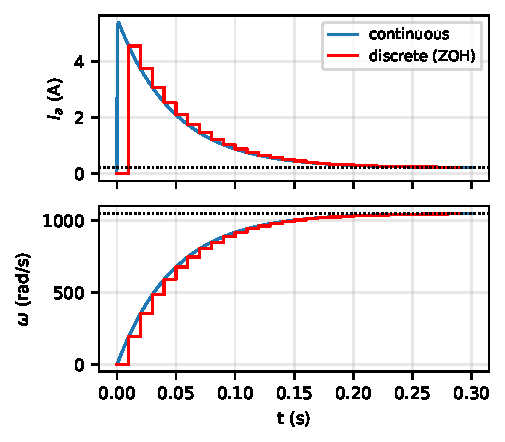
\includegraphics[width=\columnwidth]{nominal.pdf}
\caption{Respuesta del modelo ajustado a \SI{12}{V}: la corriente se estabiliza en \SI{0.2}{A} y la velocidad en \SI{1047}{rad/s}.}
\label{fig:nominal}
\end{figure}

\begin{figure}[!t]
\centering
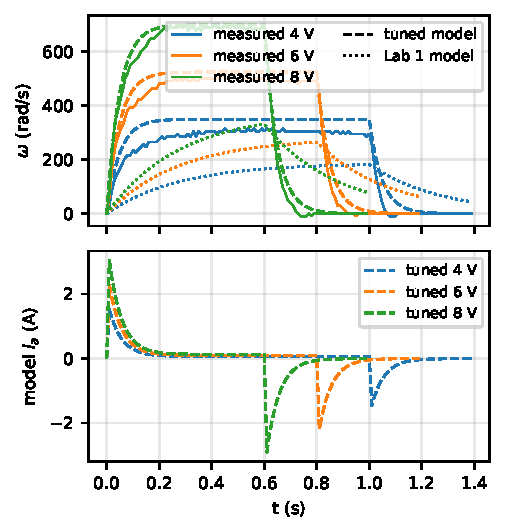
\includegraphics[width=\columnwidth]{ajuste.pdf}
\caption{Escalones de 4, 6 y \SI{8}{V} medidos en el codo, comparados con el modelo del Lab 1 (punteado) y con el modelo ajustado (discontinuo).}
\label{fig:ajuste}
\end{figure}

El modelo ajustado reproduce la constante de tiempo medida, pero sobrestima la velocidad en unos \SI{40}{rad/s} a \SI{4}{V}. Las velocidades estables medidas (305, 496 y \SI{687}{rad/s}) crecen unos \SI{96}{rad/s} por voltio, y al extrapolarlas a \SI{12}{V} dan $\approx\SI{1070}{rad/s}$, casi la velocidad nominal. Sin embargo, la recta no pasa por el origen: hay una zona muerta de unos \SI{0.8}{V} debida a la fricción seca de la caja y del brazo, que un modelo lineal no puede representar.

\section{Diseño de los observadores}
\subsection{Luenberger}
La matriz de observabilidad $\mathcal{O}=[C;\,CA]$ tiene rango 2, por lo que el sistema es observable midiendo solo la velocidad. El diseño inicial, con polos en $z=0.3$ y $0.4$, producía corrientes estimadas negativas de hasta \SI{-3.5}{A} con los datos reales (Fig.~\ref{fig:polos}). La razón es que el polo eléctrico de la planta ya está en $z\approx0$: llevarlo a $0.3$ hace el modo de corriente del observador más lento que el de la planta, y el pequeño error del modelo (la fricción) se acumula en la corriente. Se eligieron entonces los polos $z=\{0,\;0.2\}$, que conservan el polo eléctrico y aceleran el mecánico, con lo que
\begin{equation}
\Phi(z)=z^2-0.2z,\qquad L=\begin{bmatrix}-0.00312\\ 0.6124\end{bmatrix}.
\end{equation}

\begin{figure}[!t]
\centering
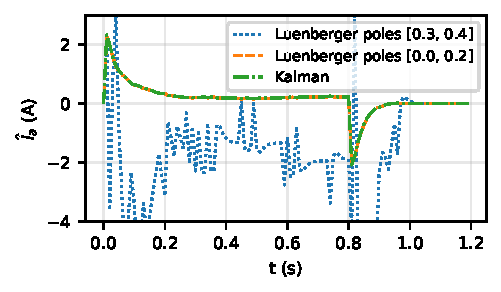
\includegraphics[width=\columnwidth]{polos.pdf}
\caption{Corriente estimada con los datos del escalón de \SI{6}{V}: con los polos $\{0.3,0.4\}$ el observador de Luenberger da corrientes negativas; con $\{0,0.2\}$ coincide con el filtro de Kalman.}
\label{fig:polos}
\end{figure}

\subsection{Kalman}
La varianza de la medición se tomó de los datos en estado estable de los escalones, entre 26 y \SI{45}{(rad/s)^2}, y se usó $R=35$. Para el modelo se dejó una incertidumbre de \SI{10}{mA} en la corriente y de \SI{10}{rad/s} en la velocidad, y para la estimación inicial se tomó una incertidumbre mayor en la corriente, que no se mide:
\begin{equation}
Q=\begin{bmatrix}10^{-4} & 0\\ 0 & 100\end{bmatrix},\quad P_0=\begin{bmatrix}0.1 & 0\\ 0 & 100\end{bmatrix}.
\end{equation}
La ganancia converge a $K=[-5.98\times10^{-4}\;\;0.771]^T$. Con estos valores no fue necesario resintonizar.

\section{Implementación}
Las matrices se calculan en Python y se escriben en un archivo de cabecera que compila el firmware. Como $C=[0\;1]$, la innovación es escalar y el filtro de Kalman no requiere invertir matrices. El paso del observador de Luenberger queda:
\begin{lstlisting}
// x(k) = (A - L C) x(k-1) + L y(k-1) + B u(k-1)
float e  = y_ant - x[1];
float x0 = AD[0]*x[0] + AD[1]*x[1] + BD[0]*u_ant + LG[0]*e;
float x1 = AD[2]*x[0] + AD[3]*x[1] + BD[1]*u_ant + LG[1]*e;
\end{lstlisting}
y la corrección del filtro de Kalman:
\begin{lstlisting}
float s  = Pm[3] + RK;            // C P- C' + R
float K0 = Pm[1]/s, K1 = Pm[3]/s; // ganancia
float e  = y - x1;                // innovacion
x[0] = x0 + K0*e;  x[1] = x1 + K1*e;
\end{lstlisting}
El lazo de \SI{10}{ms} incluye la medición, los dos observadores, el actuador y el envío de los datos.

\section{Resultados}
\subsection{Simulación con datos medidos}
Antes de la implementación se ejecutaron los dos observadores, con el mismo algoritmo del firmware, sobre los escalones medidos (Fig.~\ref{fig:sim}). En los tres escalones el error RMS de la velocidad fue de 12--14~rad/s para Luenberger y de 2.6--3.1~rad/s para Kalman. Las corrientes estables estimadas coincidieron entre ambos métodos (0.27, 0.23 y \SI{0.19}{A} a 4, 6 y \SI{8}{V}).

\begin{figure}[!t]
\centering
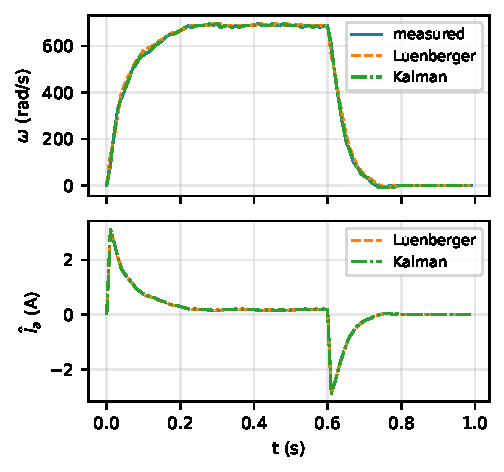
\includegraphics[width=\columnwidth]{simulacion.pdf}
\caption{Simulación de los observadores sobre el escalón medido de \SI{8}{V}.}
\label{fig:sim}
\end{figure}

\subsection{Implementación en la Pico}
La Fig.~\ref{fig:escalon} muestra un escalón de \SI{5}{V} estimado en tiempo real. Ambos observadores siguen la velocidad medida, y la corriente estimada presenta el pico de arranque (\SI{1.9}{A}), se estabiliza en \SI{\approx0.25}{A} y se vuelve negativa durante el frenado.

\begin{figure}[!t]
\centering
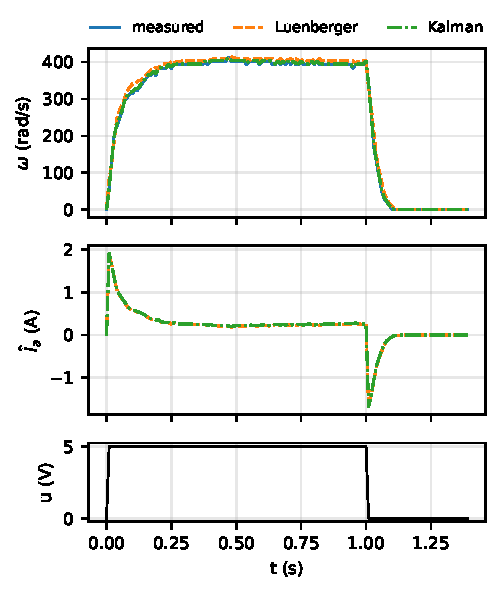
\includegraphics[width=\columnwidth]{real_escalon.pdf}
\caption{Implementación en la Pico: escalón de \SI{5}{V} durante \SI{1}{s}.}
\label{fig:escalon}
\end{figure}

Ante cambios de referencia de 4, 8, 3, $-6$ y \SI{-3}{V} (Fig.~\ref{fig:perfil}), los observadores siguen la velocidad en todos los tramos, incluida la inversión de giro. La corriente estimada muestra un pico en cada cambio de referencia y llega a \SI{-3}{A} al invertir el giro, que es el comportamiento esperado de un motor DC.

\begin{figure}[!t]
\centering
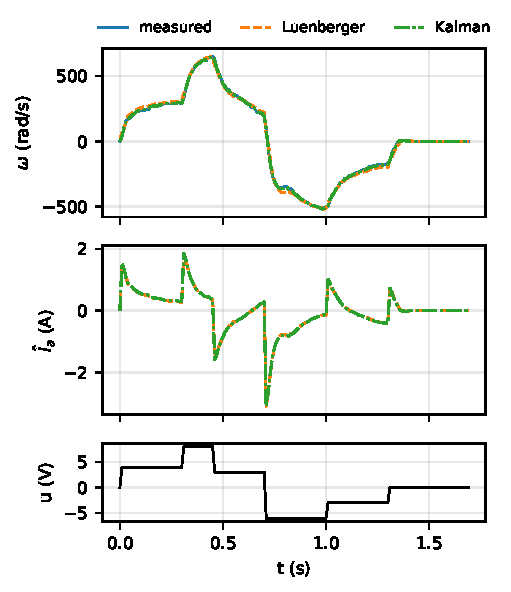
\includegraphics[width=\columnwidth]{real_perfil.pdf}
\caption{Cambios de referencia: 4, 8, 3, $-6$, $-3$ y \SI{0}{V}.}
\label{fig:perfil}
\end{figure}

Para la prueba de perturbación, el codo va y viene a $\pm\SI{3.5}{V}$ durante \SI{6}{s}, invirtiendo el giro al llegar a 0.5 y \SI{1.4}{rad}, mientras el antebrazo se frena con la mano (Fig.~\ref{fig:pert}). Cada vez que se aplica la carga, la velocidad medida cae y la corriente estimada sube de \SI{\approx0.4}{A} a 1.0--\SI{1.3}{A}. Ese valor se acerca a la corriente de bloqueo a \SI{3.5}{V} ($3.5/R_a\approx\SI{1.6}{A}$). La Tabla~\ref{tab:rms} resume los errores.

\begin{figure}[!t]
\centering
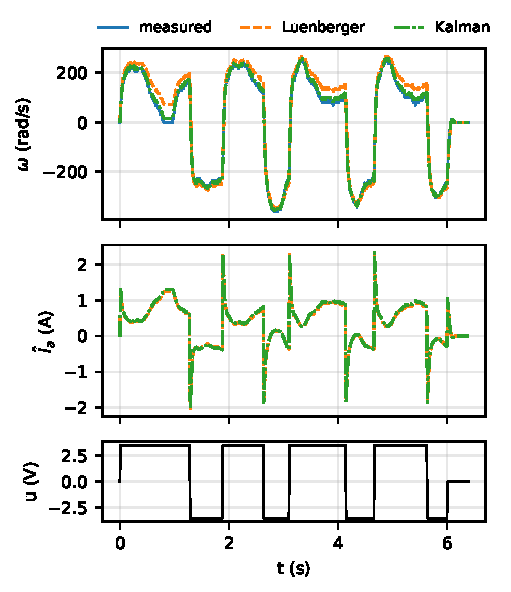
\includegraphics[width=\columnwidth]{real_perturbacion.pdf}
\caption{Perturbación: el codo va y viene a $\pm\SI{3.5}{V}$ y se frena con la mano en tres ocasiones.}
\label{fig:pert}
\end{figure}

\begin{table}[!t]
\centering
\caption{Error RMS de la velocidad estimada (\si{rad/s})}
\label{tab:rms}
\begin{tabular}{lcc}
\toprule
Prueba & Luenberger & Kalman \\
\midrule
Escalones 4, 6 y \SI{8}{V} (simulación) & 12--14 & 2.6--3.1 \\
Perturbación de carga (Pico) & 34.8 & 7.8 \\
\bottomrule
\end{tabular}
\end{table}

\section{Discusión}
El ajuste del modelo fue necesario: el modelo del Lab~1 no cumplía la condición nominal porque su resistencia de armadura era unas 30 veces mayor de lo esperado. Al fijar $K_v$ y $\beta$ con las condiciones de estado estable y ajustar solo $J$ y $L_a$, el modelo cumple la especificación del fabricante y reproduce la dinámica medida. El error remanente se debe a la fricción seca, que no es lineal.

En el observador de Luenberger, la elección de los polos resultó determinante. Con $T_s=\SI{10}{ms}$ el modo eléctrico de la planta es prácticamente instantáneo, y un polo del observador lejos de $z=0$ vuelve muy sensible la estimación de la corriente a los errores del modelo. El filtro de Kalman, en cambio, calcula su ganancia a partir de $Q$ y $R$, sin elegir polos a mano, y se comportó bien desde el primer diseño.

Con el motor frenado, la velocidad estimada no llega a cero (Fig.~\ref{fig:pert}): ninguno de los dos modelos incluye el par de carga, así que el observador espera que con voltaje aplicado el motor gire. Kalman sufre menos este sesgo porque su ganancia sobre la velocidad ($0.77$) le da más peso a la medición. Una mejora natural sería agregar el par de carga como un tercer estado.

En la práctica también apareció una limitación del montaje: al invertir el giro con el motor a alta velocidad, el pico de corriente y la energía que devuelve el motor apagaban la fuente de alimentación. Por eso se limitaron los experimentos a inversiones de $\pm\SI{6}{V}$ o menos dentro de la zona media del recorrido del codo.

\section{Conclusiones}
\begin{itemize}
\item Con una sola medición de velocidad, ambos observadores reconstruyen la corriente de armadura de forma coherente, tanto en estado estable como en los transitorios y ante cargas.
\item El filtro de Kalman sigue la velocidad unas cuatro veces mejor que el observador de Luenberger bajo perturbaciones (7.8 frente a \SI{34.8}{rad/s} RMS) y filtra el ruido de cuantización del encoder.
\item El diseño de Luenberger depende de los polos elegidos. Conviene conservar en $z\approx0$ los modos que son mucho más rápidos que el periodo de muestreo.
\item La Raspberry Pi Pico ejecuta los dos observadores y la adquisición en un lazo de \SI{10}{ms} sin dificultad, lo que la hace una alternativa económica a la tarjeta myRIO.
\end{itemize}

\begin{thebibliography}{9}
\bibitem{guia} M. Giraldo, ``Laboratory 4: State observers and estimators,'' Control Digital, Universidad EIA, 2026.
\bibitem{guiaeia} J. Cossio, S. Neumann y M. A. Giraldo, ``Guía práctica para la implementación de observadores de estado discretos,'' Universidad EIA.
\bibitem{pololu} Pololu Corporation, ``37D Metal Gearmotors,'' hoja de datos, rev. 1.2.
\bibitem{ogata} K. Ogata, \emph{Ingeniería de control moderna}, 5\textsuperscript{a} ed. Prentice Hall, 2010.
\bibitem{welch} G. Welch y G. Bishop, ``An introduction to the Kalman filter,'' UNC Chapel Hill, 1995.
\end{thebibliography}

\end{document}
